%!TEX root = ../../thesis.tex
\graphicspath{{Chapters/appendix_nascomp/figures/}}
\chapter{CVPRNAS NAS Competitions}\label{chap:nascomp}

\section{Introduction}
\added{
While looking at ways to evaluate BonsaiNet and SpiderNet, it began to become of interest to consider what exactly
constitutes a `good' NAS  algorithm. In literature, NAS algorithms are almost exclusively evaluated over well-known
benchmark datasets like CIFAR-10 and ImageNet. By this metric, the best NAS algorithms are the ones that do best over these specific datasets;
these are the algorithms that get extensively cited and are used as measuring sticks for subsequent algorithms. This becomes
a positive feedback loop as good performance on these specific datasets becomes more and more synonymous with `good NAS
algorithm', which in turn raises the performance necessary for publication. The work to evalute BonsaiNet and SpiderNet
was often guilty of the same problem; the focus frequently narrowed to just these benchmark datasets, and the original
aim of NAS was forgotten. For the longest time the mantra was ``97\%+ on CIFAR-10 and it is publishable", without considering
whether the broader scope. The entire NAS field had boiled down to a leaderboard, where the only
metric of importance was performance on the two computer vision benchmarks.}

\added{
However, the real world use case of NAS was still a pressing concern; NAS is for novel problems and tasks, where
the best practices were unknown. It is for problems where the cumulative decades of research might not apply, and when
there is not much time to spend researching potential candidates. This disconnect between the answers to the questions of
\textit{``What makes a good NAS algorithm?''} and \textit{``How should a NAS algorithm be used?''} became glaringly,
unavoidably obvious. Even worse, that disconnect gave rise to a more troubling question:
Do NAS algorithms work in the real world, or are they simply tailored to these existing datasets?}

\added{
With that realization, it was important to devise a way to bring the former two questions into agreement,
and find an answer to the latter; and this process took the form of two NAS competitions held at CVPR-NAS 2021 and 2022.}

\section{Competition Design}
\added{
The general idea of the competition was to separate the design of a NAS algorithm from the datasets it will run over,
such that the search algorithm design was not specifically tailored to the dataset it would run over. To do this,
competitors were asked to design components of a NAS pipeline, the specific breakdown of which is shown in
Table~\ref{tab:nascomp_pipeline_components}.}

\begin{table}[h]
\begin{center}
\begin{tabular}{c|c|c}
Component & NASComp-2021 & NASComp-2022 \\
		  \hline
Data Preprocessing & Fixed 			& User-designed \\
Data Augmentation  & Fixed			& User-designed \\
Search Algorithm   & User-designed	& User-designed \\
Training Policy    & Fixed			& User-designed \\
\end{tabular}
\end{center}
\caption[NASComp pipeline components]{The NASComp pipeline components for the 2021 and 2022 editions of the competition,
broken down by whether they were supplied by us, the organizers (fixed) or by the competitor (user-designed).}
\label{tab:nascomp_pipeline_components}
\end{table}
\added{
The user-submitted components would be plugged into the server-side NAS pipeline, which would then pass each server-side
dataset through the pipeline, thus searching for and training one model per dataset. The datasets were kept secret and
permanently server-side, meaning that competitors had no idea the contents of the datasets that they were being evaluated over.}

\added{
Competitors were then scored on
how their best test accuracy compared against a ResNet-18:}
\begin{align}
	\text{Dataset Score 2021} &= 10 \cdot \frac{\text{Accuracy} - \text{ResNet accuracy}}{100 - \text{ResNet accuracy}}  &\\
	\text{Dataset Score 2022} &= 10 \cdot \max \left(\frac{\text{Accuracy} - \text{ResNet accuracy}}{100 - \text{ResNet accuracy}}, -1 \right)
\end{align}

\added{
Therefore, a perfect 100\% test accuracy was worth 10 points, a test accuracy equivalent to ResNet-18 was worth 0 points, and
negative points were scored for test accuracies lower than ResNet-18. The final submission score was the sum of all individual
dataset scores. This motivated trying to balance performance across all $n$ datasets, as good performance in one dataset
could be wiped out by poor performance in another.}


\section{Datasets}
\added{
Crucial to the conceit of the competitions was the creation of novel datasets, such that no ``best-practices'' existed
for any of the datasets involved in the competition, meaning competitors could not necessarily submit something like a
ResNet and expect high quality results. Furthermore, it meant that since the datasets were entirely unknown and unseen,
competitors could not tailor their submissions to the particular nuances of the datasets. To reduce the scope
of the task being asked of the competitors, each of the datasets used for the competition was structured
as image classification tasks, that is, given some four-dimensional tensor of size [batch, channel, height, width], classify
each image in the batch into one of $n$ classes. Competitors were given a per-dataset metadata file that contained
minimal information regarding the dataset, namely, its shape, total number of images, number of classes in the classification
problem, and the benchmark ResNet-18 score.}

\section{2021 Datasets}
\added{
Six datasets were used or developed for the 2021 edition of the competition, divided into 3 \textit{development} datasets
and 3 \textit{evaluation} datasets. The former were given to competitors directly to test their algorithms with,
while the latter were held secret until after the competition.}

\subsection{AddNIST}
\begin{figure}[h]
	\centering
	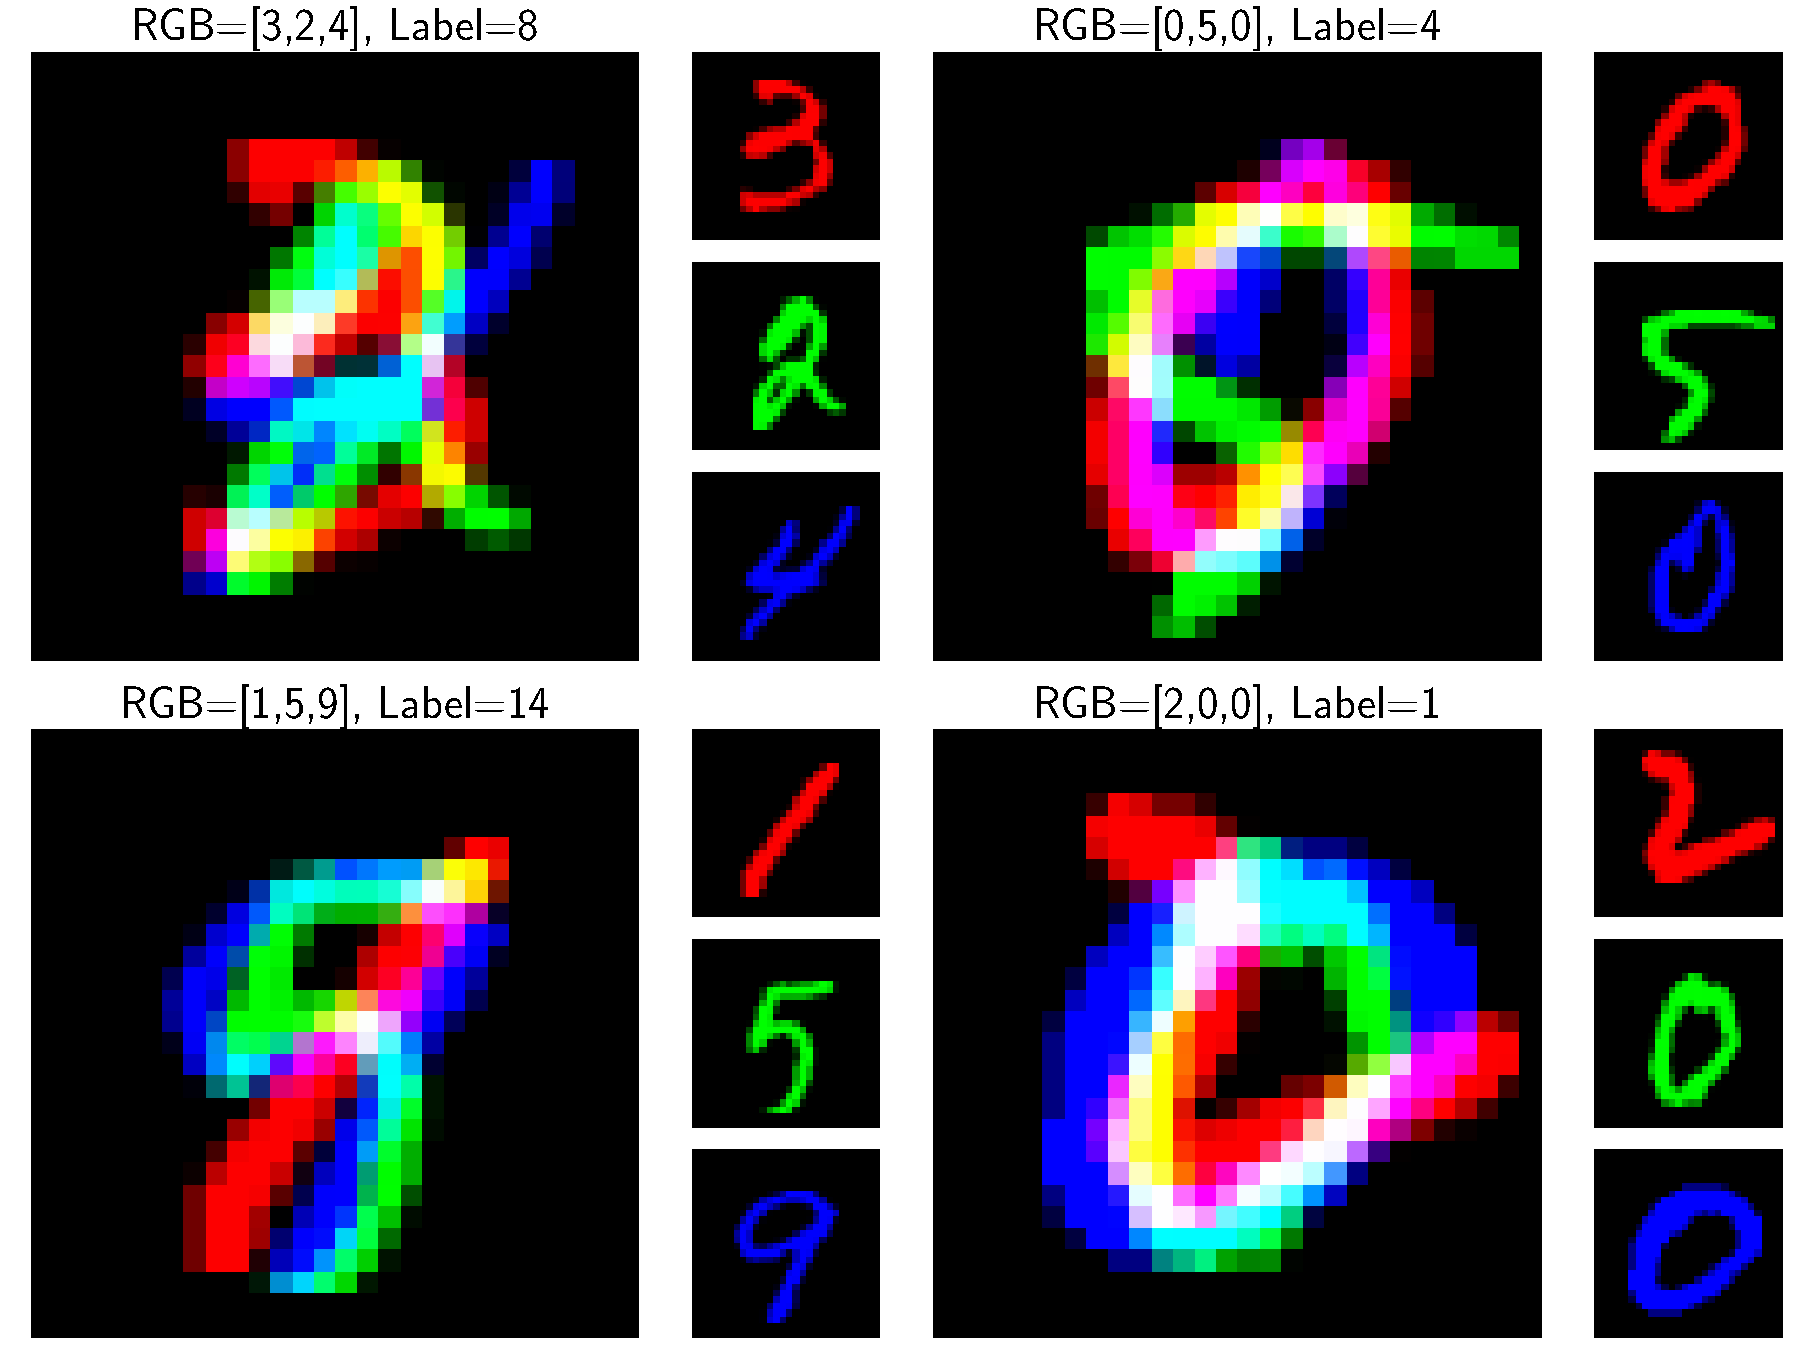
\includegraphics[width=.6\textwidth]{AddNIST}
	\caption{An example of the AddNIST data}
    \label{fig:addnist}
\end{figure}
\added{
The first development dataset was called AddNIST. Each image contains three MNIST images, one in each of the RGB channels.
The output class is $(r + g + b) - 1$, where $r$, $g$, and $b$ refer to the digits represented by the three MNIST images.
The three images are chosen such that $(r+g+b)-1 < 20$. The train and validation split use Torch MNIST train images,
while test split uses test images. Combinations are chosen at random, but weighted such that each of the 20 classes are
evenly represented in both data splits. Each of the three component MNIST images are normalized according to the MNIST
mean and standard deviation before they are combined into the 3 image datapoints. See Figure~\ref{fig:addnist} for examples.
Our benchmark model scored a 92.08\% on this dataset, and the submission record was 95.06\%, achieved by Atech AutoML.}

\subsection{FashionMNIST}
\added{
The second development dataset was just FashionMNIST\citep{xiao2017}, see Figure~\ref{fig:language and fashion}a for examples.
Our benchmark model scored a 92.87\% on this dataset, and the submission record was a 94.44\%, achieved by Atech AutoML.}

\begin{figure}[ht]
	\centering
	\begin{subfigure}{.48\textwidth}
		\centering
		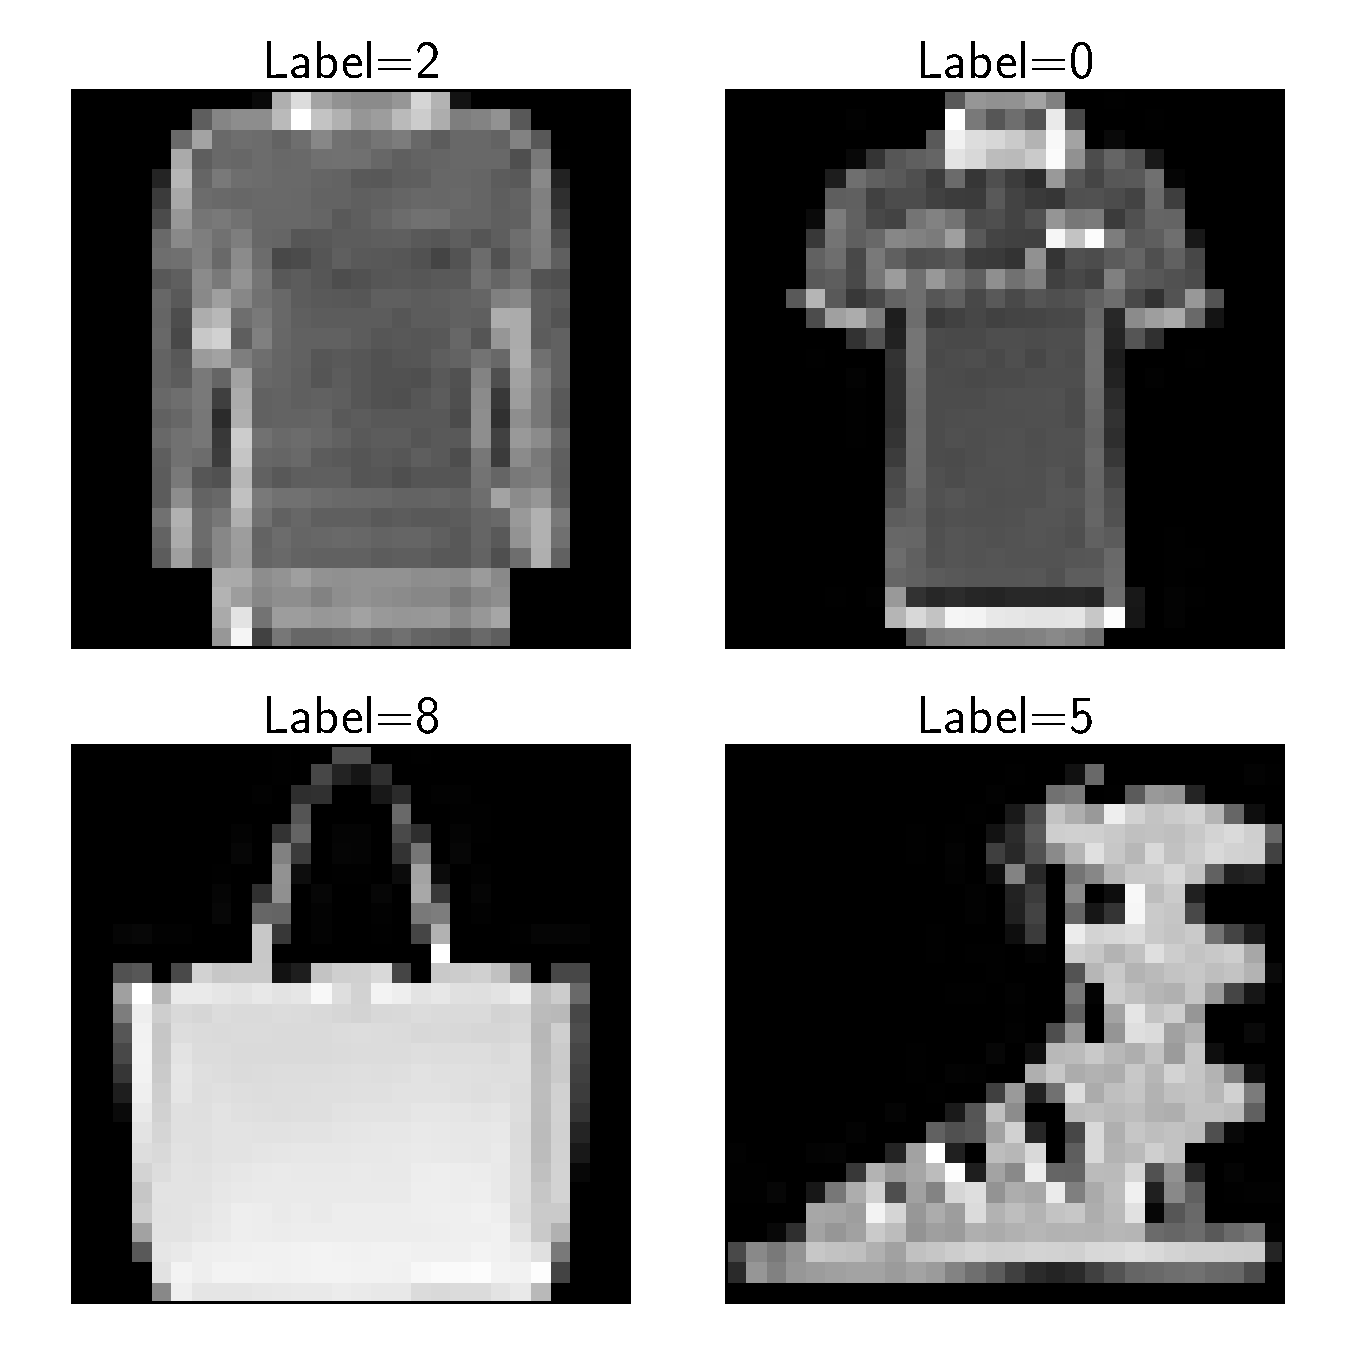
\includegraphics[width=.9\textwidth]{fashionmnist}
		\caption{FashionMNIST data}
	\end{subfigure}
	\begin{subfigure}{.48\textwidth}
		\centering
		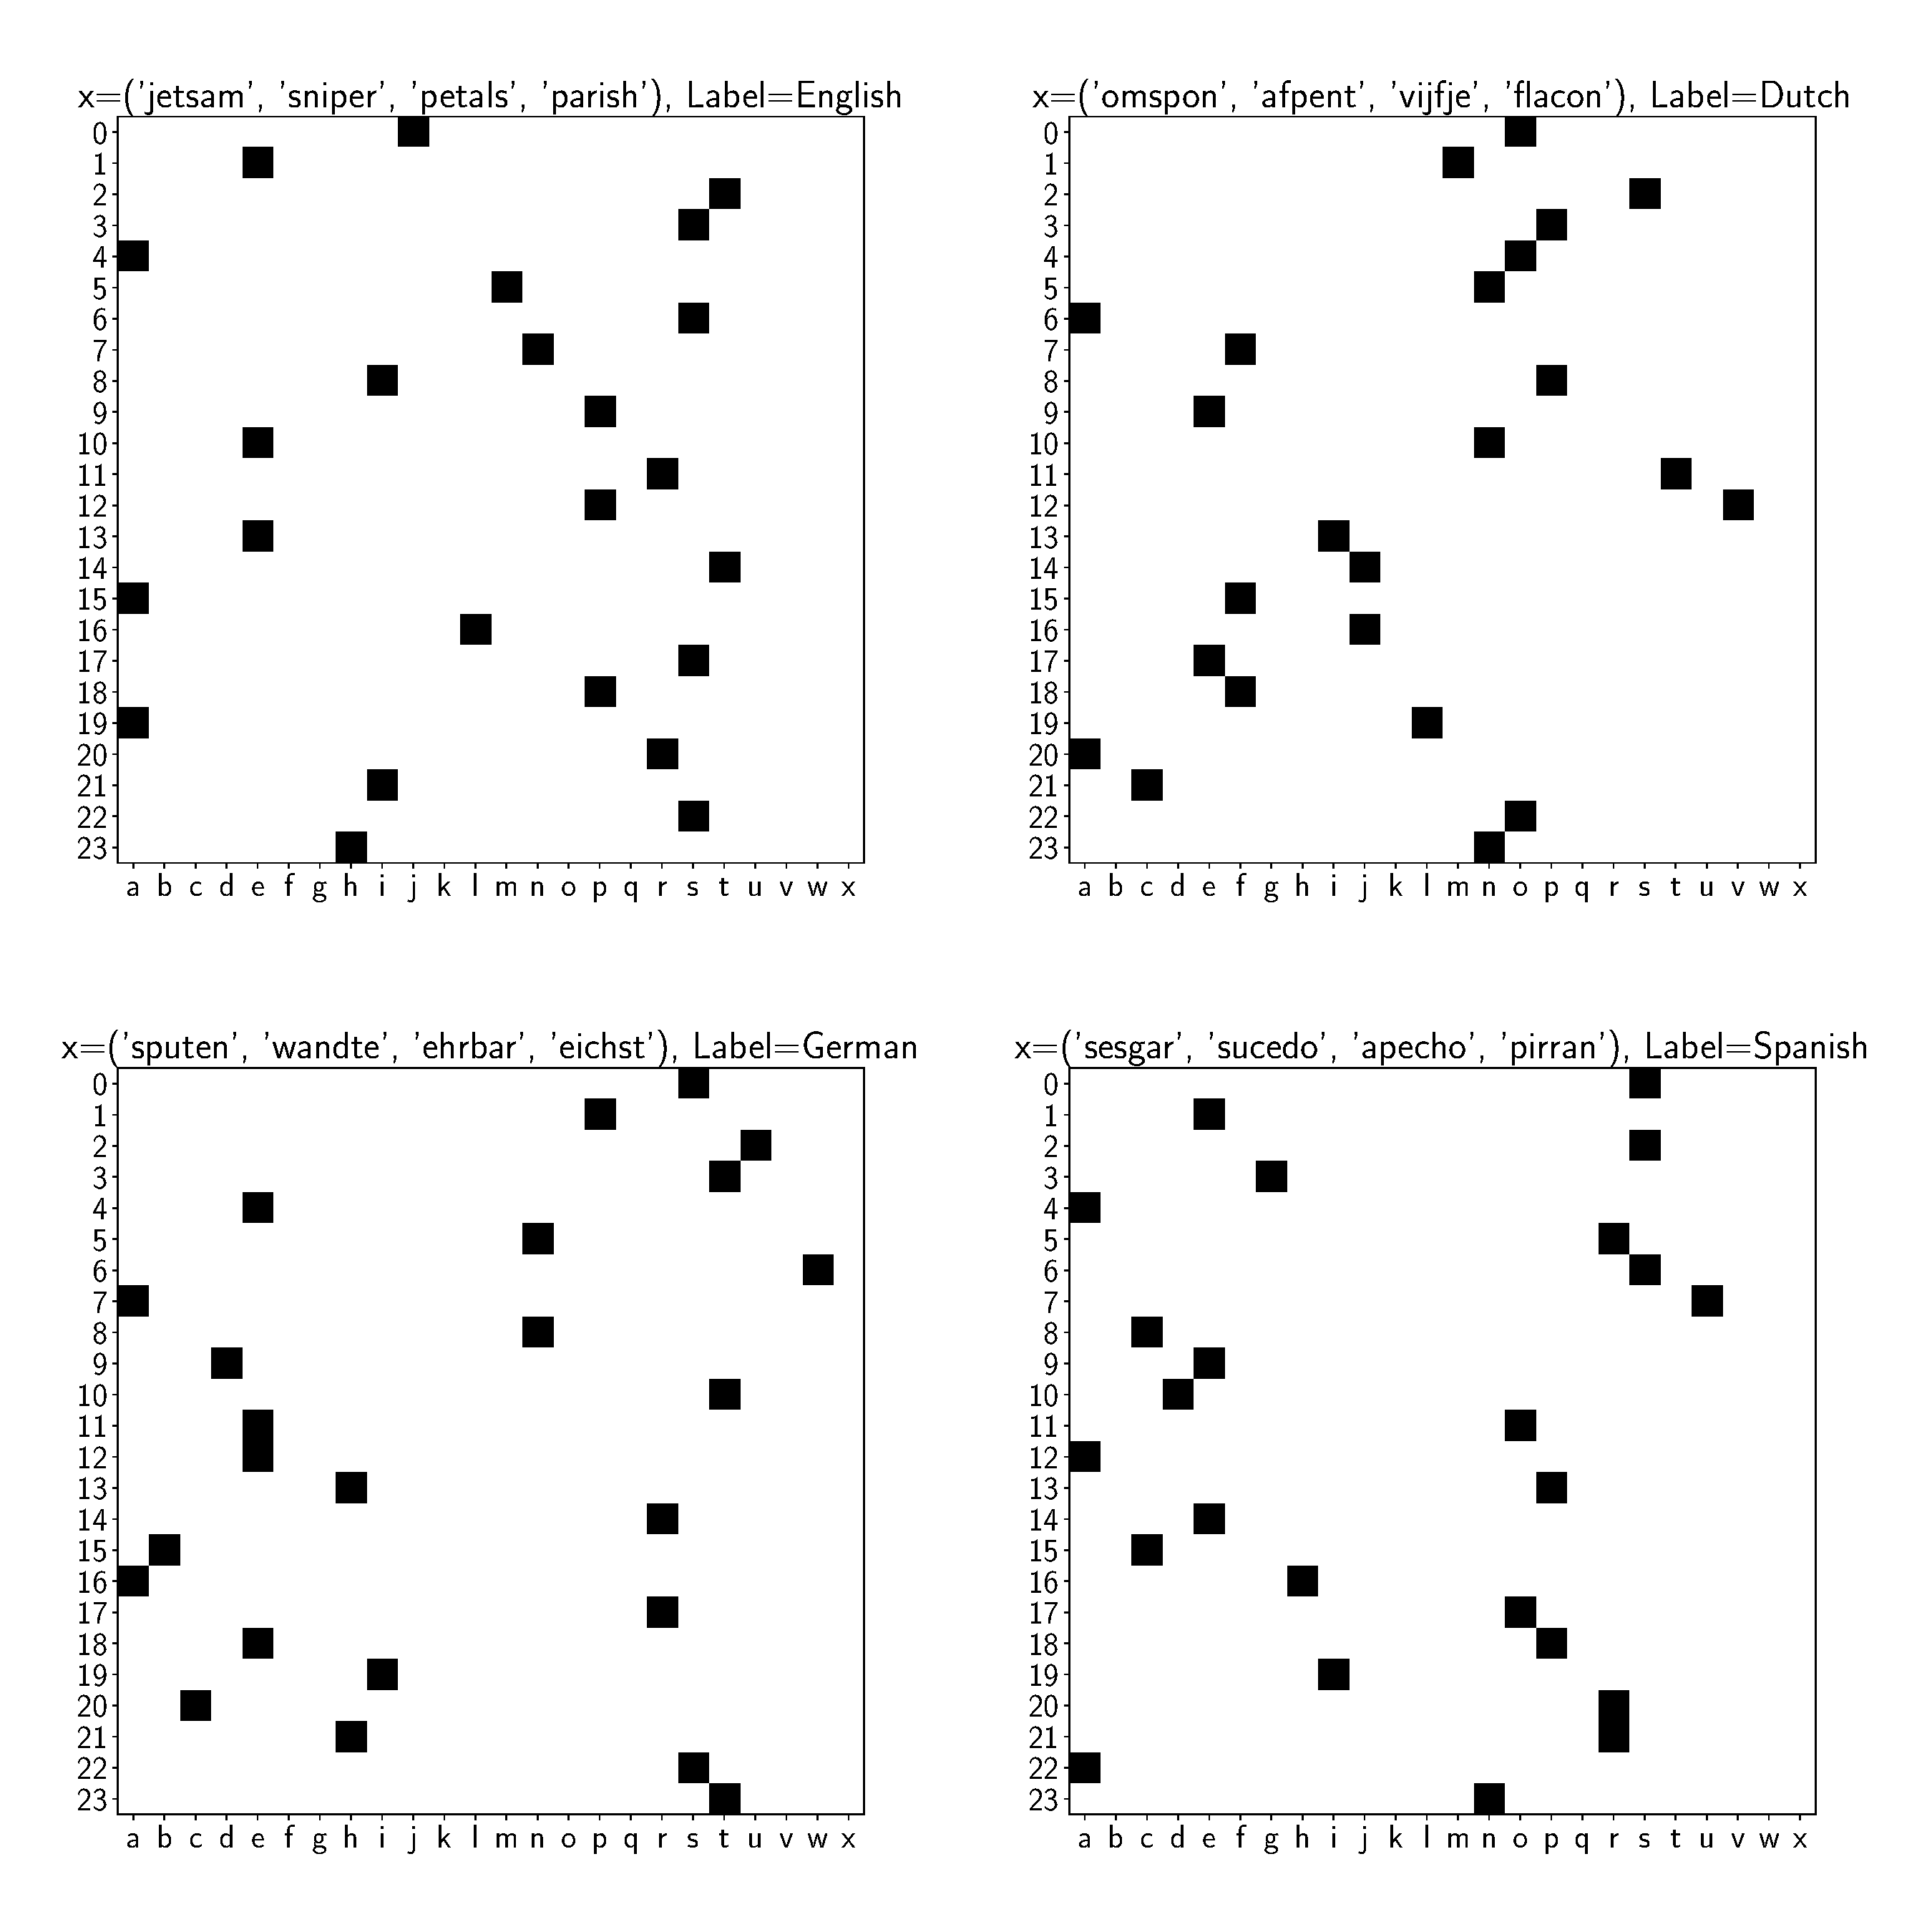
\includegraphics[width=.9\textwidth]{langugage}
		\caption{Language identification data}
	\end{subfigure}
	\caption[The FashionMNIST and Language datasets]{The FashionMNIST and Language datasets.}
	\label{fig:language and fashion}
\end{figure}

\subsection{Language}
\added{
The third development dataset was codenamed language. Here, we loaded the Aspell language dictionary for 10 languages
that all use the Latin alphabet: English, Dutch, German, Spanish, French, Portuguese, Swedish, Zulu, Swahili, and Finnish.
We then filtered these words to only those that use 6 letters total. Of these six letter words, all that used diacritics
(letters such as é or ü), y, or z were removed, meaning there were 24 possible letters within each word. These words
were then combined into random groups of 4, and one hot encoded. This creates a 24x24 matrix, which constitutes the
input image. The six letter words were divided into train and test groups to prevent train/test leakage, meaning that
there were no words shared across the train and test word sets used to generate the train and set images. The image class
refers to the original language that the four words come from. See Figure~\ref{fig:language and fashion}b for examples. Our benchmark model scored an 87.00\% on this dataset,
and the submission record was 89.71\%, achieved by `yonga`. We were surprised by how well models could learn this data,
given how random it looks to the human eye.}

\subsection{MultNIST}
\added{
The first evaluation dataset was codenamed MultNIST. The process of this is very similar to AddNIST, except the output
class is $(r*g*b) \mod 10$; the last digit of the product of `r`, `g`, and `b`. All other processing is identical
to that of AddNIST. Our benchmark model scored a 91.55\% on this dataset, and the submission record was 95.45\%, achieved by Atech AutoML.}

%\begin{figure}[ht]
%	\centering
%	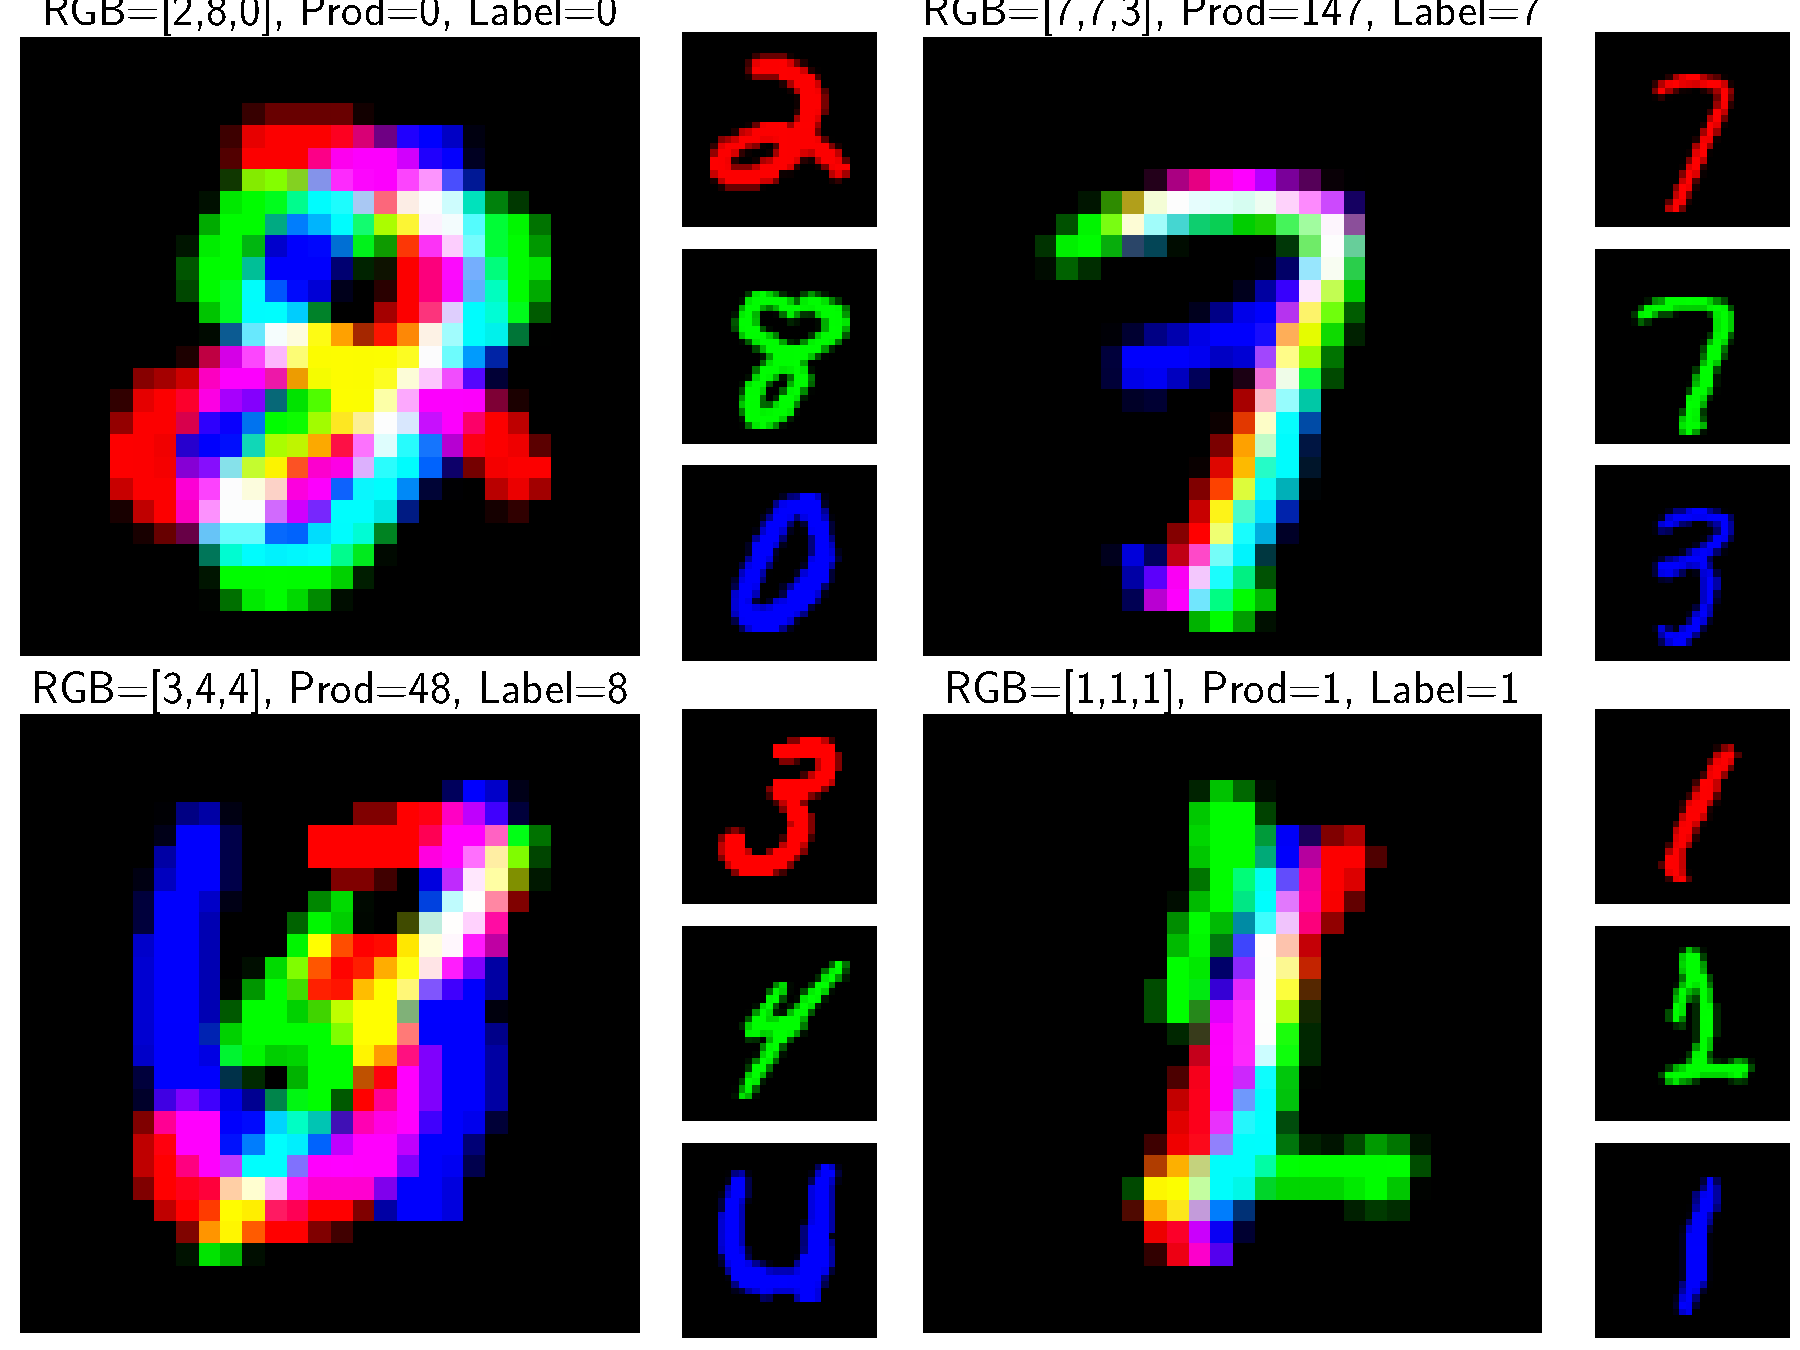
\includegraphics[width=.6\textwidth]{multnist}
%	\caption{An example of the MultNIST data}
%    \label{fig:multnist}
%\end{figure}


\subsection{CIFARTile}
\begin{figure}[ht]
	\centering
	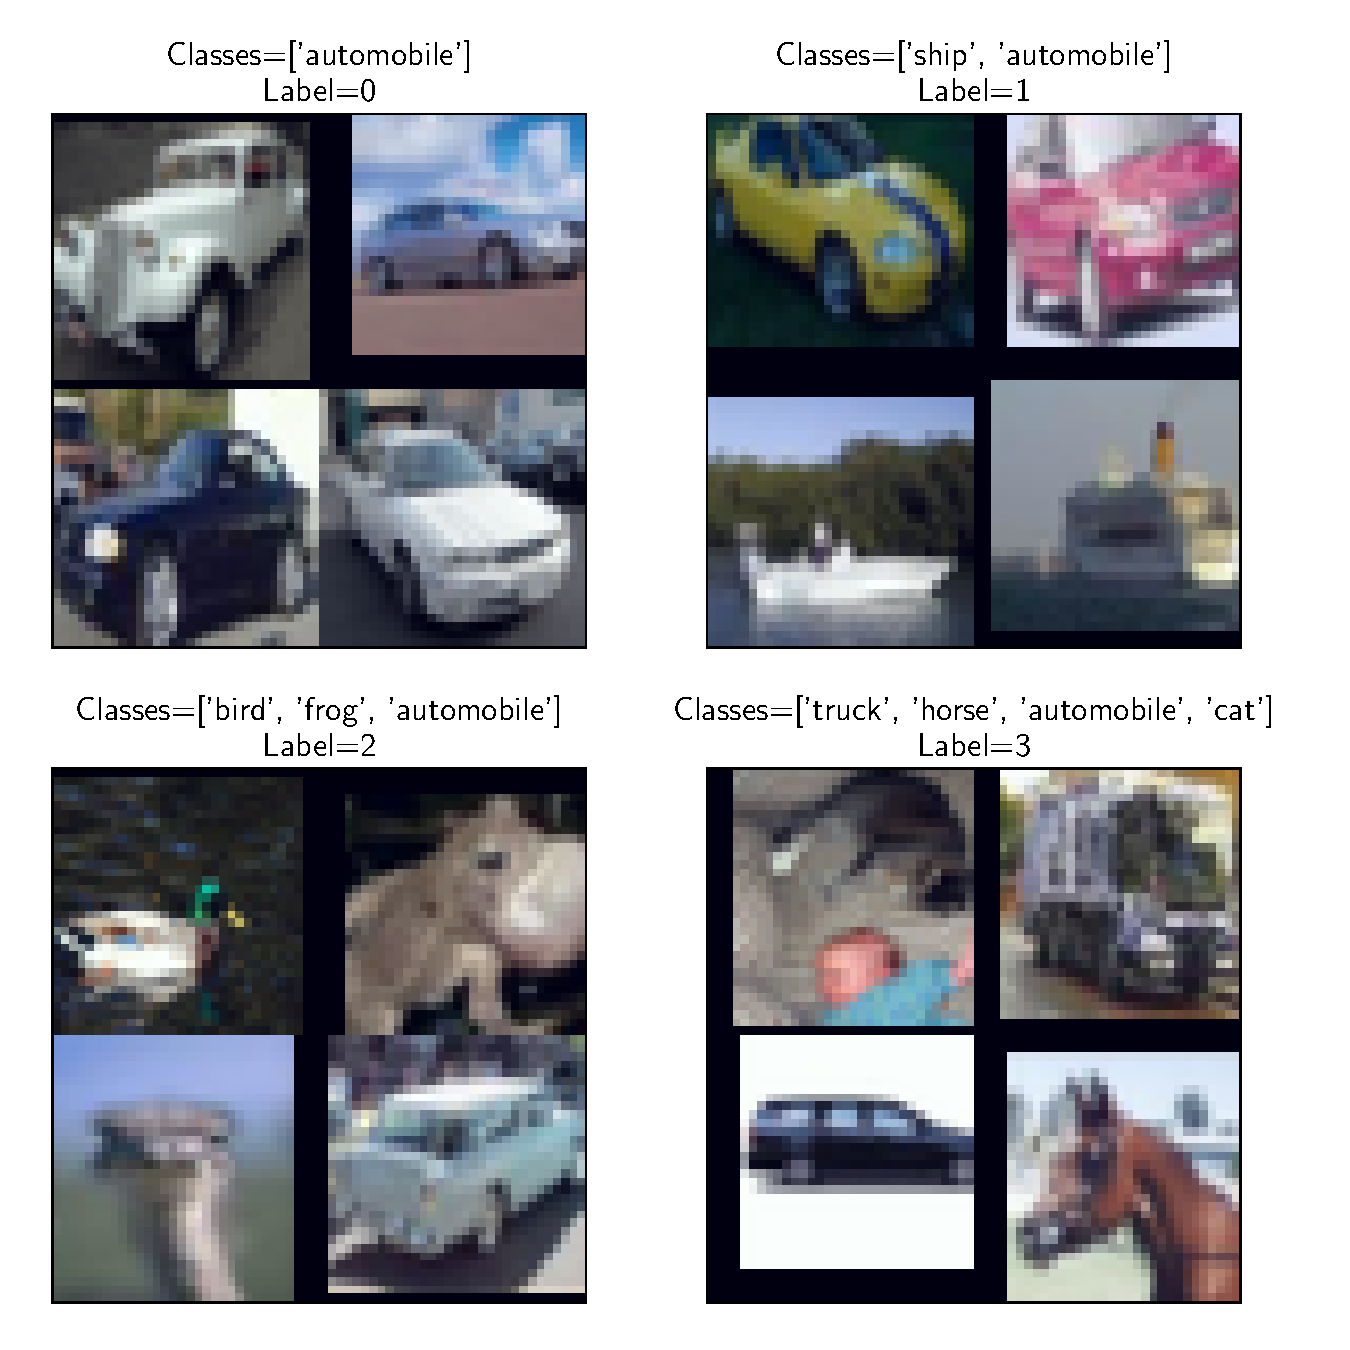
\includegraphics[width=.7\textwidth]{cifartile}
	\caption{An example of the CIFARTile data}
    \label{fig:cifartile}
\end{figure}
\added{
The second evaluation dataset was codenamed CIFARTile. This takes images from CIFAR-10 and tiles them into a 2x2 grid.
The label for the grid is the total number of discrete classes in the tiling minus 1 (to ensure that the classes are
`0, 1, 2, 3`]. So for example, a tile of `[horse, horse, frog, cat]` has three discrete classes and thus has a label of 2.
The train and validation data splits get images from the train set of CIFAR-10, while the test data split gets
images from the test set.}
\added{
For each grid, a total number of classes `nclasses` is chosen between 1 and 4. If `nclasses` is:}

\begin{enumerate}
	\item 1 class is selected at random and all four images in the tile are from that one class.
	\item 2 classes are selected at random, and there are two images of each class in the tile, placed randomly into the tiling.
	\item 3 classes are selected at random. There are two images of the first class and one of the second and third, with the images placed randomly into the tiling.
	\item 4 classes are selected at random. There is one image of each class, placed randomly into the tiling.
\end{enumerate}
\added{
Each individual image in the tile is processed as per the recommended CIFAR-10 augmentation and normalization policy
used in the PyTorch documentation: a 32 pixel random crop with padding 4, a random horizontal flip, and a normalization
around the global channel mean and standard deviation. See Figure~\ref{fig:cifartile} for examples. Our benchmark model
scored a 45.56\% on this dataset, and the submission record was 73.08\%, achieved by SRCB VC Lab.}

\subsection{Gutenberg}
\begin{figure}[h]
	\centering
	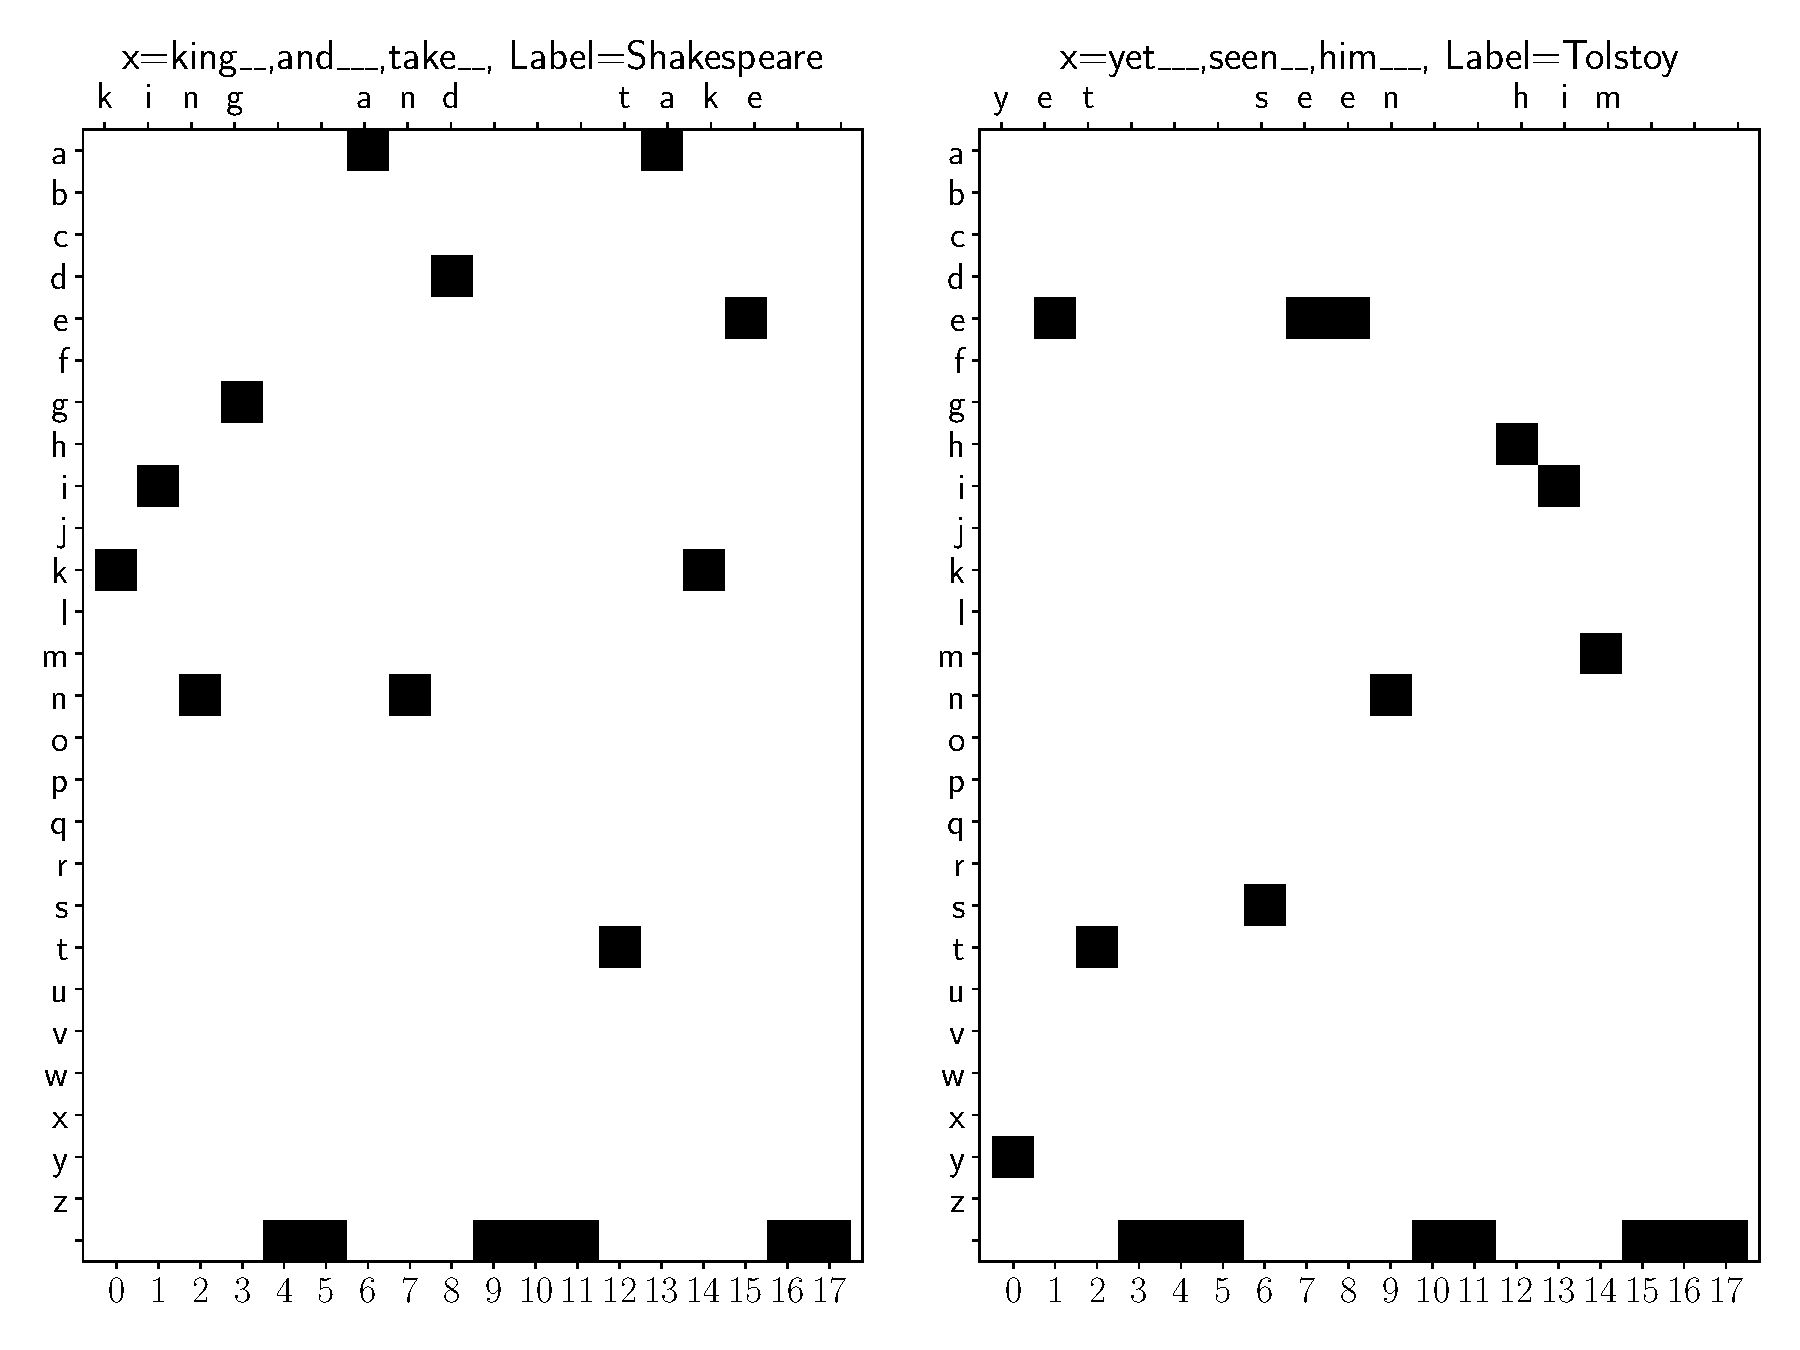
\includegraphics[width=.8\textwidth]{gutenberg}
	\caption{Examples of the Gutenberg data}
    \label{fig:gutenberg}
\end{figure}
\added{
The third evaluation dataset was codenamed Gutenberg. Here, the following texts were downloaded from Project Gutenberg (CITATION) from six different authors:}

\begin{itemize}
	\item \textbf{Thomas Aquinas}: Summa I-II, Summa Theologica Part III, On Prayer and the Contemplative Life
	\item \textbf{Confucius}: The Sayings of Confucius, The Wisdom of Confucius
	\item \textbf{Hawthorne}: The Scarlet Letter, The House of the Seven Gables
	\item \textbf{Plato}: The Republic, Symposium, Laws
	\item \textbf{Shakespeare}: Romeo and Juliet, Macbeth, Merchant of Venice, King Lear, Twelfth Night
	\item \textbf{Tolstoy}: War and Peace, Anna Karenina
\end{itemize}
\added{
Each text was an English translation of the source material, with authors chosen to represent a wide variety of cultures,
time periods, and languages. From each text, basic text preprocessing is performed; removing punctuation, mapping diacritics
to their base letters, and removing common 'structure' words (things like "chapter", "scene" or "prologue". The texts were
then split into sequences of words. From these word sequences, consecutive sequences of three words that were between 3
and 6 letters long were extracted, called "phrases". Phrases that appeared in multiple authors' corpuses were removed.
Each word in each phrase were padded with underscores if they were shorted than 6 letters. For example, for Shakespeare,
you might have something like \texttt{such\textunderscore\textunderscore sweet\textunderscore sorrow} or
\texttt{lady\textunderscore \textunderscore doth\textunderscore\textunderscore protest}. These phrases were then
one-hotted, and the label corresponds to the original author that wrote the phrase. See Figure~\ref{fig:gutenberg} for examples.
Our benchmark model scored a 40.98\% on this dataset, and the submission record was 50.85\%, achieved by Atech AutoML.}

\section{2022 Datasets}
\added{
For the the 2022 competition, the five novel 2021 datasets (AddNIST, MultNIST, Language, Gutenberg, and CIFARTile) were
used as development datasets, and three new evaluation datasets were designed.}

\subsection{Sadie}
\added{
The first of the 2022 evaluation datasets was codenamed Sadie, as reference to the satellite imagery the dataset was
derived from. The Sadie dataset used the BigEarthNet dataset~\citep{sumbul2019} as a foundation, but does not use the original
land-cover classification labels provided alongside the dataset. Instead, Sadie takes advantage that the BigEarthNet patches are taken
from images of 10 distinct European countries (Austria, Belgium, Finland, Ireland, Kosovo, Lithuania, Luxembourg, Portugal, Serbia, Switzerland)
to instead modify the task into  a country identification problem. This is done by identifying the Sentinel~\citep{Sentinel} patch
from which the BigEarthImage was cropped, and then cross-referencing the coordinates of that patch with a map of Europe.
Following this process, 10,000 images from each country were extracted from BigEarthNet, see Figure~\ref{fig:sadie} for examples.
The ResNet-18 benchmark scored 80.33\% accuracy, and the competition record of 96.08\% was attained by the Sun Yat-sen University team.}

\begin{figure}[h]
	\centering
	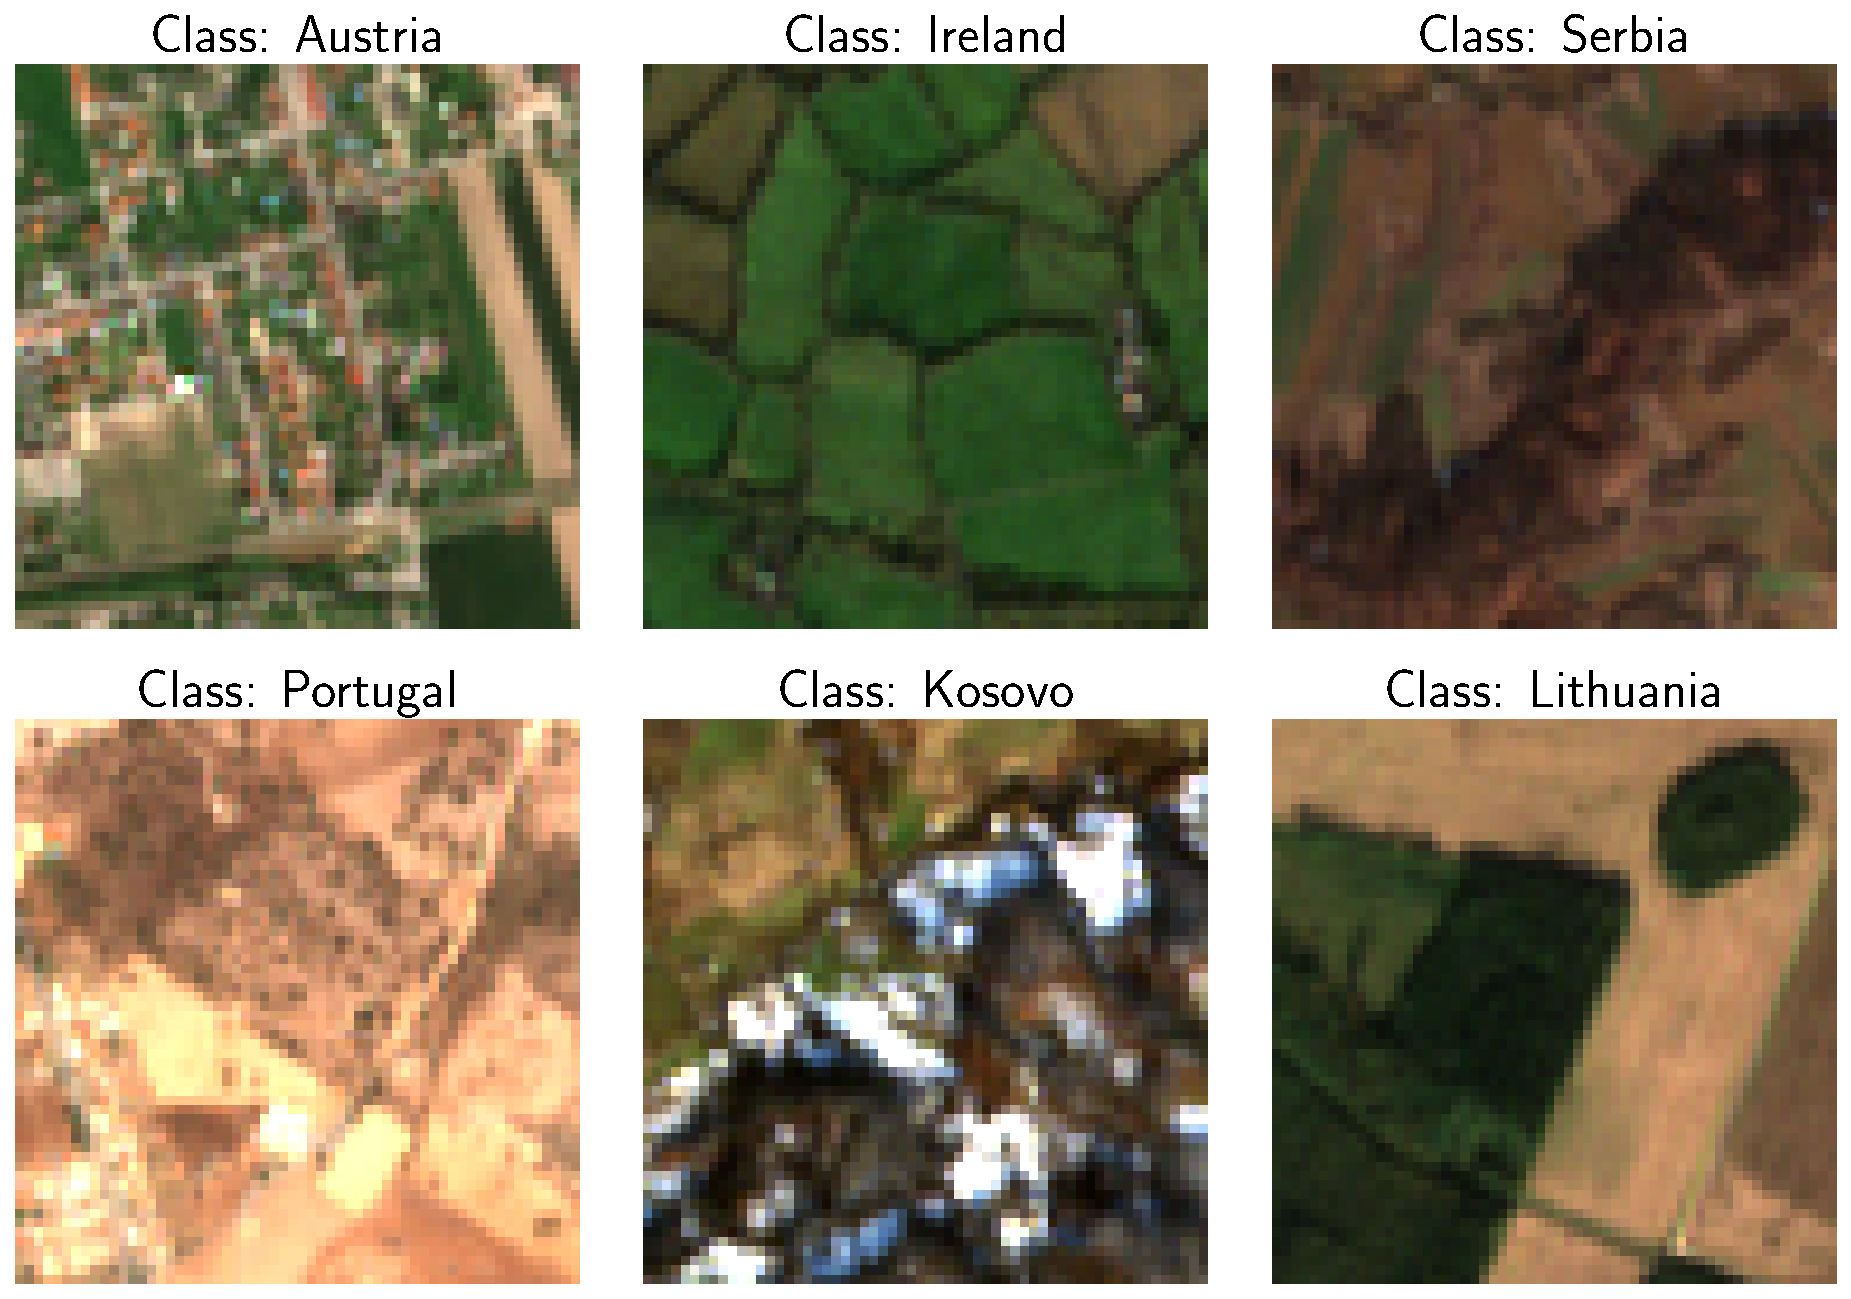
\includegraphics[width=.8\textwidth]{sadie}
	\caption{Examples of the Sadie dataset}
    \label{fig:sadie}
\end{figure}

\subsection{Chester}
\added{
The second evaluation dataset was codenamed Chester, as reference to the chess games from which the dataset was sourced.
Here, all recorded games from Chess.com that involved one of 8 grandmasters (Bobby Fischer, Garry Kasparov, Magnus Carlsen, Viswanathan Anand,
Hikaru Nakamura, Anatoly Karpov, Fabiano Caruana, and Mikhail Tal) were scraped. From each of those games, the final 15\% of
board states were extracted, where the $n$th board state refers to the particular positioning of pieces after $n$ moves.
Then, the boards were one-hot encoded by piece type and color, creating a 12\texttimes8\texttimes8 tensor. The task was then
to predict the final game outcome (white win, draw, black win) from the 12-channel input image, and some examples can be seen in
Figure~\ref{fig:chester}. The ResNet-18 benchmark scored 57.826\% accuracy, and the competition record of 62.98\%
was again attained by the Sun Yat-sen University team.}

\begin{figure}[h]
	\centering
	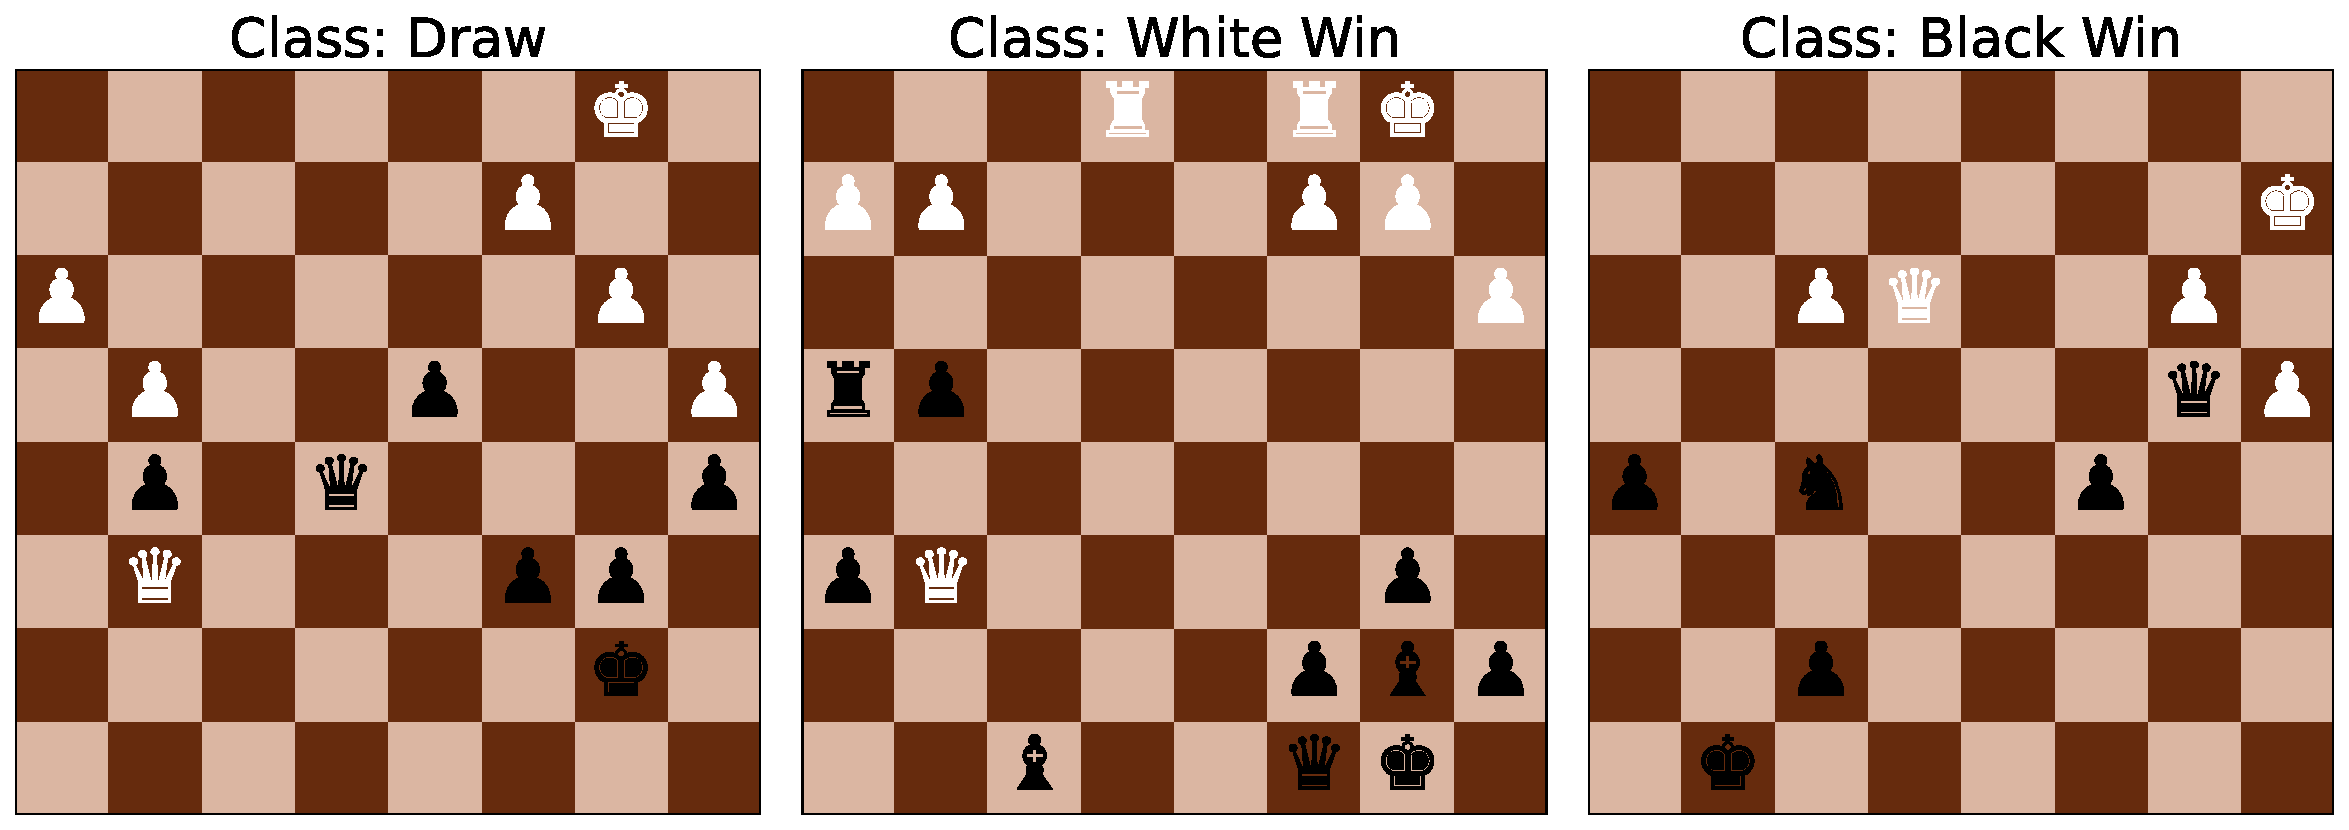
\includegraphics[width=.8\textwidth]{chester}
	\caption{Examples of the Chester dataset}
    \label{fig:chester}
\end{figure}

\subsection{Isabella}
\added{
The final evaluation dataset was codenamed Isabella, from the Isabella Stewart Gardner museum in Boston that published
the data. Here, recordings of concerts from within the ISG museum were downloaded from the museum website~\citep{ISG}, each
labeled by era of composition, i.e, Baroque, Classical, Romantic, and 20th Century. The recordings were then split into
non-overlapping 5 second snippets, each of which were converted into spectrograms, examples of which can be seen in
Figure~\ref{fig:isabella} The task was to predict which of the four compositional eras the particular spectrogram belonged to.
An error in the metadata specifications for this dataset meant that competitors were told that the dataset had 6 labels as
opposed to the correct 4, which potentially might negatively skew results. In fairness, all benchmarks of this thesis' work
as well as any general results using the Isabella dataset will also use the incorrect 6-class format.
The ResNet-18 benchmark scored 62.02\% accuracy, which no competitor was able to beat. The closest was again the
Sun Yat-sen University team, who scored a 61.42\% accuracy.}

\begin{figure}[h]
	\centering
	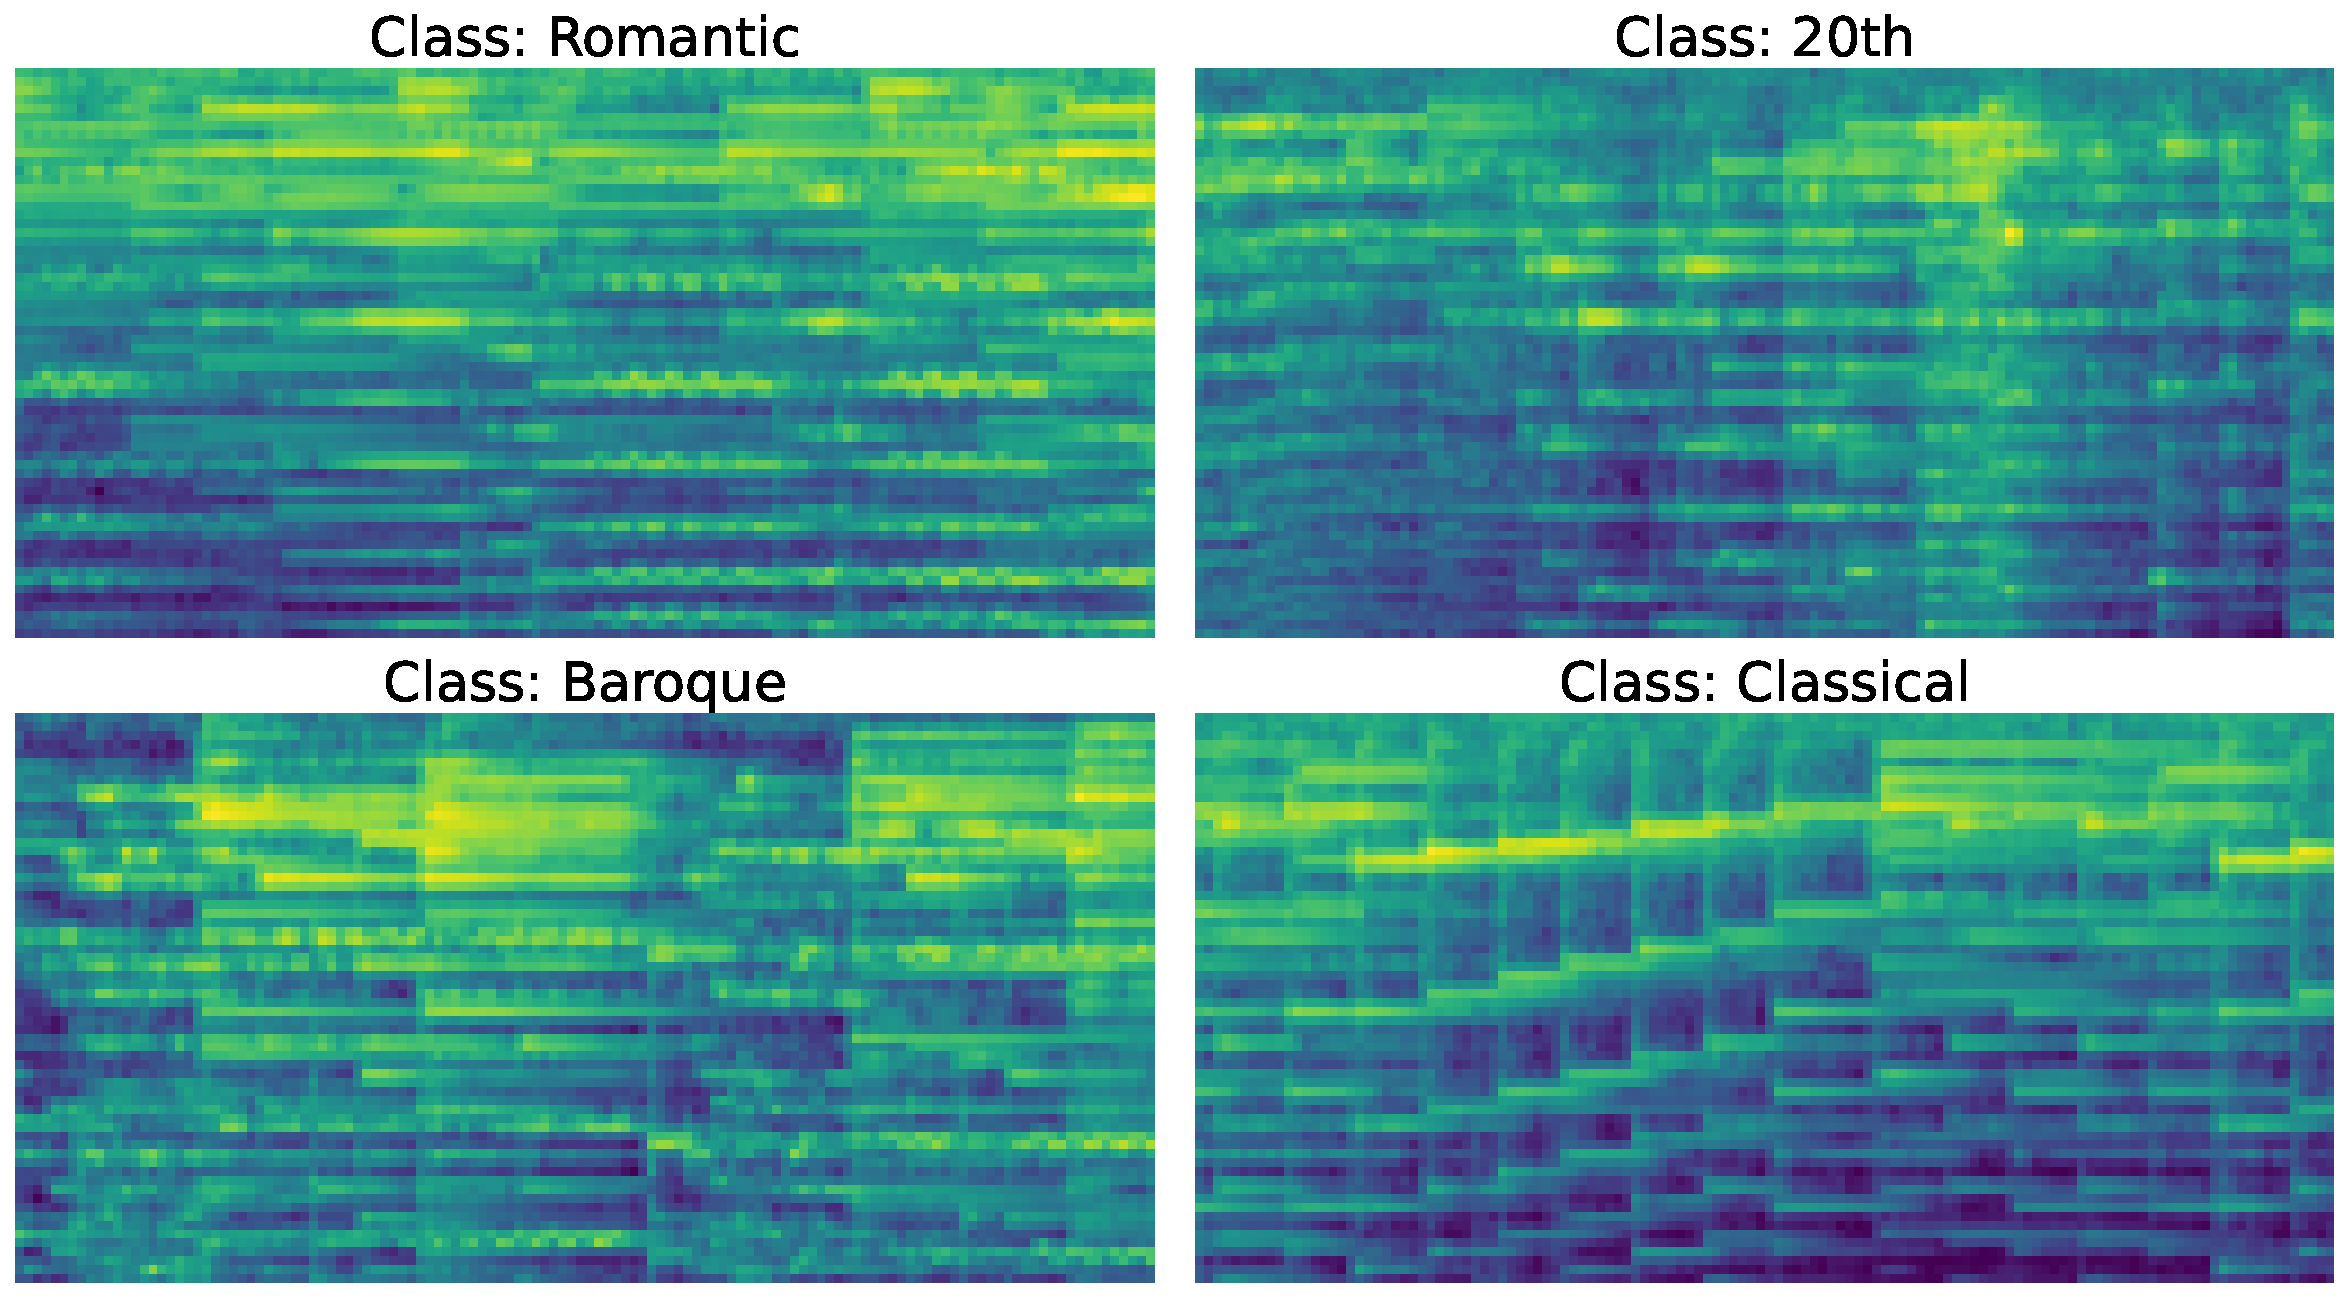
\includegraphics[width=.8\textwidth]{isabella}
	\caption{Examples of the Isabella dataset}
    \label{fig:isabella}
\end{figure}

\section{Competition Engagement}
\added{
The 2021 competition saw 75 entrants, 341 total submissions, and 11 teams qualify for the final competition phase over
the 3 evaluation datasets. The Samsung Research Center Beijing team won the competition, with the University of Friedburg
team coming in second, and Kakao Enterprise coming in third, and all three teams were invited to speak at the CVPR-NAS 2021
workshop.}

\added{
The 2022 edition saw lesser engagement (likely due to the absence of an offered cash prize), but the competition still received
around 25 entries, with the Sun Yat-sen University team being the only team to successfully qualify through to the final round,
and thus were winners by default.}

